\documentclass[10pt,a4paper]{article}
\usepackage[utf8]{inputenc}
\usepackage{amsmath}
\usepackage{amsfonts}
\usepackage{amssymb}
\usepackage[left=2cm,right=2cm,top=2cm,bottom=2cm]{geometry}
\usepackage{url}
\usepackage{graphicx}
\usepackage[per-mode=symbol]{siunitx}

\begin{document}
\title{IDEAS SimpleHouse exercise instructions}
\author{Filip Jorissen, KU Leuven}
\maketitle

\section*{Introduction}
The goal of this exercise is to become familiar with 
Modelica and the IDEAS library. 
Since the IDEAS library components are typically used
by combining several components graphically, the use of 
equation falls outside of the scope of this exercise.\\

For this exercise you will create a model of a simple house,
consisting of a heating system, one building zone 
and a ventilation model. 
The exercise starts from a template file that should 
not produce any errors. This file will be extended in
several steps, adding complexity.
In between each step the user should be able to simulate the
model. I.e. no errors should be produced and simulation results 
may be compared.\\

Prerequisites are that you should have the latest version of Dymola
installed. You should have a working compiler, and a license. 
Dymola can be downloaded from 
\url{http://www.3ds.com/products-services/catia/products/dymola/trial-version/}. 
Installation instructions for Dymola and a C-compiler can be found on 
\url{http://www.3ds.com/fileadmin/PRODUCTS/CATIA/DYMOLA/PDF/Installation.pdf}.
The latest version from the IDEAS library should be downloaded and opened in Dymola. 
To verify you installation try to simulate \path{IDEAS.Fluid.Actuators.Dampers.Examples.Damper} by opening the simulation tab (bottom right) and by clicking simulate (
\includegraphics[scale=0.5]{simulate.png}).\\

In the following sections the simple house model is discussed 
in several steps. 
Each step first qualitatively explains the model part.
Secondly the names of the required IDEAS models 
are listed.
Thirdly we provide high-level instructions of how to
set up the model.
If these instructions are not clear immediately, 
have a look at the model documentation and at the type of
connectors the model has, 
try out some things, 
make an educated guess, etc.
Finally we provide reference results that allow you to check
if your implementation is correct. 
Depending on the parameter values that you choose, results
may differ.
 



\section{Building wall model}
\paragraph{Qualitative discussion}
Even though one of the goals of IDEAS is to provide
detailed building envelope models, a very simple building
envelope model will be constructed manually using thermal
resistors and heat capacitors.
The house consists of a wall represented 
by a single heat capacitor and a thermal resistor. 
The thermal resistor and boundary temperature 
are already added in the template.
The wall has a surface area of A\_wall = 100 $m^2$, 
a thickness of d\_wall = 25 cm
\footnote{We suggest to declare these parameters in the equation section similar to the example, but this is not required.}, 
a thermal conductivity of k\_wall = 0.04 W/mK, 
a density of rho\_wall = 2000.
The heat capacity value of a wall may be computed as $C=A\cdot d \cdot c_p \cdot rho$.

\paragraph{Required models}
In this first step only the Modelica Standard Library (MSL) 
model \path{Modelica.Thermal.HeatTransfer.Components.HeatCapacitor}
is required.

\paragraph{Connection instructions}
Connect the heat capacitor to the thermal resistor.

\paragraph{Reference result}
If you correctly added the model, connected it to the resistor and 
added the parameter values for $C$
\footnote{Double-click on a component to see a list of its parameters. Gray values indicated default values.}
then you should be able to simulate the model.
To do this, go to the simulation tab (see bottom right),
open the simulation options (`setup')
and set the model `stop time' to 1e6 seconds.
You can now simulate the model.
You can plot individual variables values by clicking on their name in the variable browser on the left.
Now plot the wall capacitor temperature value `T'. 
It should look like Figure~\ref{fig:res1}.

\begin{figure}
\centering
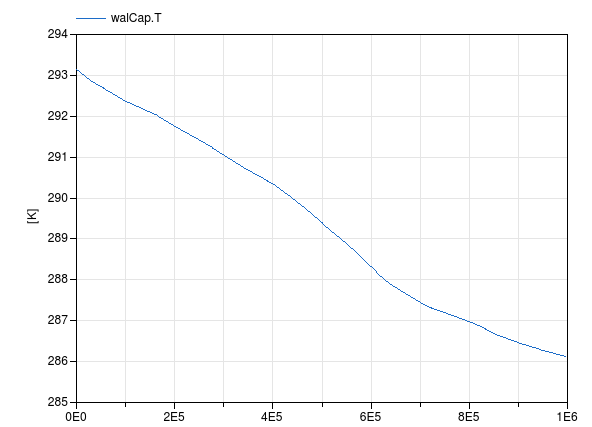
\includegraphics[scale=0.7]{result1.png}
\caption{Wall temperature in K as function of time in seconds}
\label{fig:res1}
\end{figure}


\section{Building window model}
\paragraph{Qualitative discussion}
The window has a surface area of 2~m$^2$. 
In this simple model we will therefore assume that two times the
outdoor solar irradiance is injected as heat onto the inside of the wall.

\paragraph{Required models}
\begin{itemize}
\item \path{Modelica.Blocks.Math.Gain}
\item \path{Modelica.Thermal.HeatTransfer.Sources.PrescribedHeatFlow}
\end{itemize}

\paragraph{Connection instructions}
To be able to use the value of the outdoor solar irradiance
you will need to access our weather data reader.
To do this, make a connection to the `weaBus' block. 
In the dialog box select `\textless add variable\textgreater' and here
select \path{HDirNor}, 
which is the direct solar irradiance on a surface
of 1 m$^2$, perpendicular to the sun rays. 

\paragraph{Reference result}
The result with and without the window model
is plotted in Figure~\ref{fig:res2}.

\begin{figure}
\centering
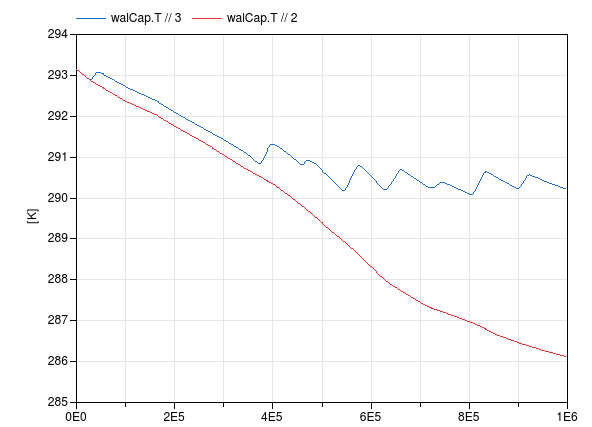
\includegraphics[scale=0.7]{result2.png}
\caption{Wall temperature in K as function of time in seconds,
with and without window}
\label{fig:res2}
\end{figure}


\section{Air model}
\paragraph{Qualitative discussion}
To increase the model detail we now add
an air model assuming the zone is 8 x 8 x 3 m in size.
The air will exchange heat with the wall.
This may be modelled using a thermal resistance 
where $R=\frac{1}{hA}$ with $A$ the heat exchange 
surface area and we choose $h=\SI{2}{\watt\per\square\meter\per\kelvin}$.


\paragraph{Required models}
\begin{itemize}
\item \path{IDEAS.Fluid.MixingVolumes.MixingVolume}
\item \path{Modelica.Thermal.HeatTransfer.Components.ThermalResistor}
\end{itemize}

\paragraph{Connection instructions}
The \path{MixingVolume} `Medium' parameter contains
information about the type of fluid and its properties
that should be modelled by the \path{MixingVolume}.
Set
\footnote{Click the right small arrow and `edit text' in the parameter dialog box, or use the Modelica text view.}
 its value to `MediumAir', which is declared in the template.

\paragraph{Reference result}
The result with and without the air model
is plotted in Figure~\ref{fig:res3}.

 

\begin{figure}
\centering
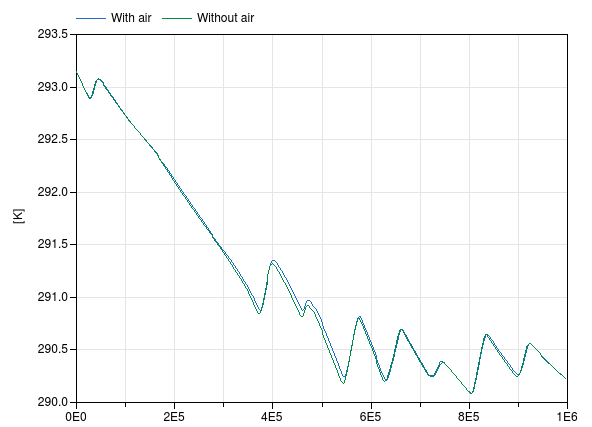
\includegraphics[scale=0.7]{result3.png}
\caption{Wall temperature in K as function of time in seconds,
with and without air model}
\label{fig:res3}
\end{figure}


\section{Heating model}
\paragraph{Qualitative discussion}
The wall temperature (and therefore the room temperature) are quite low. 
In this step a heating system is added to resolve this.
It consists of a radiator, a pump and a heater.
The radiator has a nominal power of \SI{3}{\kilo\watt} 
for a temperature difference of \SI{20}{\kelvin} between inlet and outlet
of the radiator.
The pump has a (nominal) mass flow rate of \SI{0.1}{\kilogram\per\second}.
Since the heating system uses water as a heat carrier fluid, 
the media for the models should be set to MediumWater.

\paragraph{Required models}
\begin{itemize}
\item \path{IDEAS.Fluid.HeatExchangers.Radiators.RadiatorEN442_2}
\item \path{IDEAS.Fluid.HeatExchangers.HeaterCooler_u}
\item \path{IDEAS.Fluid.Movers.FlowControlled_m_flow}
\item \path{IDEAS.Fluid.Sources.Boundary_pT}
\item \path{Modelica.Blocks.Sources.Constant}
\end{itemize}

\paragraph{Connection instructions}
Since the heating system uses water as a heat carrier fluid, 
the media for the models should be set to MediumWater.

Pressure difference modelling may be disregarded since the chosen pump
sets a fixed mass flow rate regardless of the pressure drop.

The \path{Boundary_pT} model needs to be used to set an absolute
pressure somewhere in the system. 
Otherwise the absolute 
pressure in the system is undefined.

The radiator contains one port for convective 
heat transfer and one for radiative heat transfer.
Connect both in a reasonable way.

Set the heater input to 1, meaning that it will
produce 1 time its nominal power.


\paragraph{Reference result}
The result of the \underline{air} temperature 
is plotted in Figure~\ref{fig:res4}.
The temperature rises very steeply since the 
wall is relatively well insulated ($k=\SI{0.04}{\watt\per\meter\per\kelvin}$)
and the heater is not disabled when it becomes too warm.



\begin{figure}
\centering
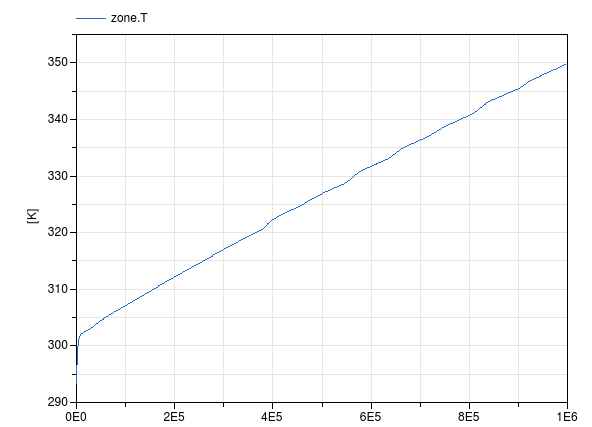
\includegraphics[scale=0.7]{result4.png}
\caption{Air temperature in K as function of time in seconds}
\label{fig:res4}
\end{figure}


\section{Heating controller model}
\paragraph{Qualitative discussion}
Since the zone becomes too warm, a controller
is required that disables the
heater when a set point is reached.
We will implement a hysteresis controller with a set point of $295.15 \pm \SI{1}{\kelvin}$ 
(21-\SI{23}{\celsius}).
A temperature sensor will measure the zone air temperature.


\paragraph{Required models}
\begin{itemize}
\item \path{Modelica.Blocks.Logical.Hysteresis}
\item \path{Modelica.Blocks.Logical.Not}
\item \path{Modelica.Blocks.Math.BooleanToReal}
\item \path{Modelica.Thermal.HeatTransfer.Sensors.TemperatureSensor}
\end{itemize}

\paragraph{Connection instructions}
The heater modulation level should be set to one when
the heater is on and to zero otherwise.


\paragraph{Reference result}
Figure~\ref{fig:res5} shows the air temperature when
the controller is added.



\begin{figure}
\centering
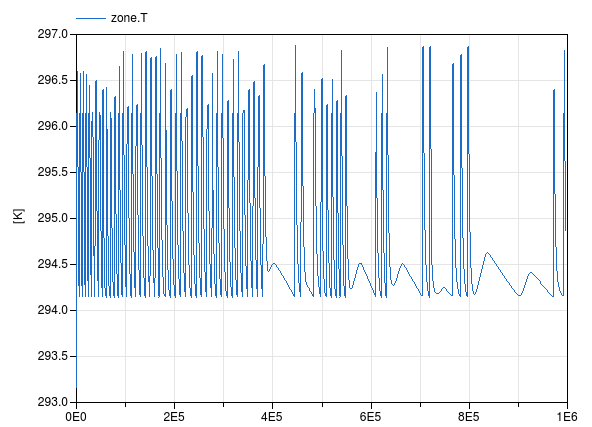
\includegraphics[scale=0.7]{result5.png}
\caption{Air temperature in K as function of time in seconds with hysteresis controller}
\label{fig:res5}
\end{figure}


\section{Free cooling model}
\paragraph{Qualitative discussion}
Finally consider that the window has a size of
6 m$^2$ instead of 2 m$^2$.
We will add a ventilation model that allows to
perform free cooling using outside air when
solar irradiation heats up the room too much.
The system consists of a fan,
a damper,
a controller with an air temperature 
set point between 23 and 25 $^{\circ}$C
and a heat recovery unit with a constant effectivity of 85\%.
Damper and fan have a nominal pressure drop of 200 Pa. 
The nominal mass flow rate of the system is 0.1 kg/s.


\paragraph{Required models}
Use some of the previously used models and in addition to this:
\begin{itemize}
\item \path{IDEAS.Fluid.HeatExchangers.ConstantEffectiveness}
\item \path{IDEAS.Fluid.Movers.FlowControlled_dp}
\item \path{IDEAS.Fluid.Actuators.Dampers.VAVBoxExponential}
\end{itemize}

\paragraph{Connection instructions}
Connect the components such that they exchange mass 
(and therefore also energy) with the \path{MixingVolume}
representing the zone air.
Add a \path{boundary_pT} to draw air from the environment.
Enable its temperature input and connect it to the `TDryBul'
variable in the weather data reader.



\paragraph{Reference result}
Figure~\ref{fig:res6} shows the result.



\begin{figure}
\centering
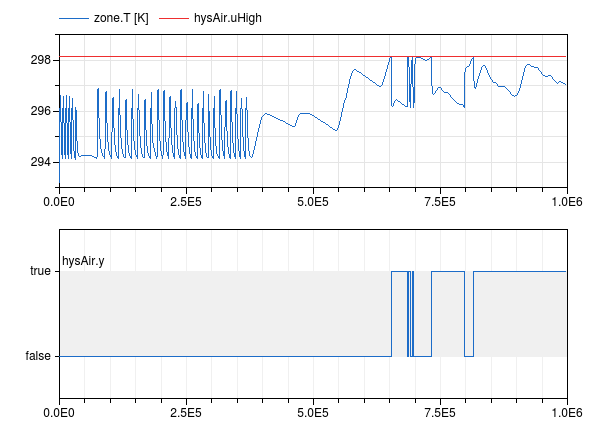
\includegraphics[scale=0.7]{result6.png}
\caption{Air temperature, hysteresis controller upper bound and hysteresis output signal as function of time in seconds}
\label{fig:res6}
\end{figure}

\end{document}